\documentclass[border=3pt]{standalone}
% Preâmbulo compartilhado pelos diagramas TikZ da aula 13 (SLAM com EKF)
\usepackage[T1]{fontenc}
\usepackage[utf8]{inputenc}
\usepackage{lmodern}
\usepackage{amsmath}
\usepackage{xcolor}
\usepackage{tikz}
\usetikzlibrary{arrows.meta,angles,quotes,decorations.pathmorphing,decorations.pathreplacing,calc,
                positioning,shapes.geometric,shapes.misc,backgrounds,fit,
                math}

% Paleta (mesma dos SVGs originais)
\definecolor{dblue}{HTML}{2A5B8C}
\definecolor{dorange}{HTML}{B3541E}
\definecolor{dgreen}{HTML}{4A7C59}
\definecolor{dred}{HTML}{9C4B4B}
\definecolor{dcream}{HTML}{F4F1EA}
\definecolor{dshade}{HTML}{DDD7C9}

% Função gaussiana (não normalizada por padrão de escala visual)
\pgfmathdeclarefunction{gauss}{3}{%
  \pgfmathparse{1/(#3*sqrt(2*pi))*exp(-((#1-#2)^2)/(2*#3^2))}%
}

% Estilos comuns (prefixo d... para não colidir com chaves internas do pgf)
\tikzset{
  >={Stealth[length=2mm]},
  dguide/.style={gray!55, dashed, line width=0.4pt},
  daxis/.style={gray!60, line width=0.7pt, ->},
  dbody/.style={fill=black!3, draw=black!80, line width=1pt},
  dacc/.style={draw=dblue, line width=1pt},
  dlbl/.style={black!55, font=\small},
  dsub/.style={black!45, font=\footnotesize},
  dstate/.style={circle, draw=black!80, fill=dcream, line width=1pt,
                 minimum size=17mm, font=\large, inner sep=1pt},
  dobs/.style={circle, draw=black!80, fill=dshade, line width=1pt,
               minimum size=14mm, font=\large, inner sep=1pt},
  dbox/.style={rounded corners=2pt, draw=black!80, fill=dcream, line width=1pt,
               align=center, inner sep=6pt},
  dop/.style={circle, draw=black!80, fill=white, line width=1pt,
              minimum size=6mm, inner sep=0pt, font=\small},
  dtrans/.style={->, dblue, line width=1pt},
  dmeas/.style={->, dorange, line width=1pt},
  dcurve/.style={line width=1pt, dblue},
  dcurveb/.style={line width=1.4pt, dorange},
}

\begin{document}
\hyphenpenalty=10000 \exhyphenpenalty=10000 \tolerance=9999 \emergencystretch=3em
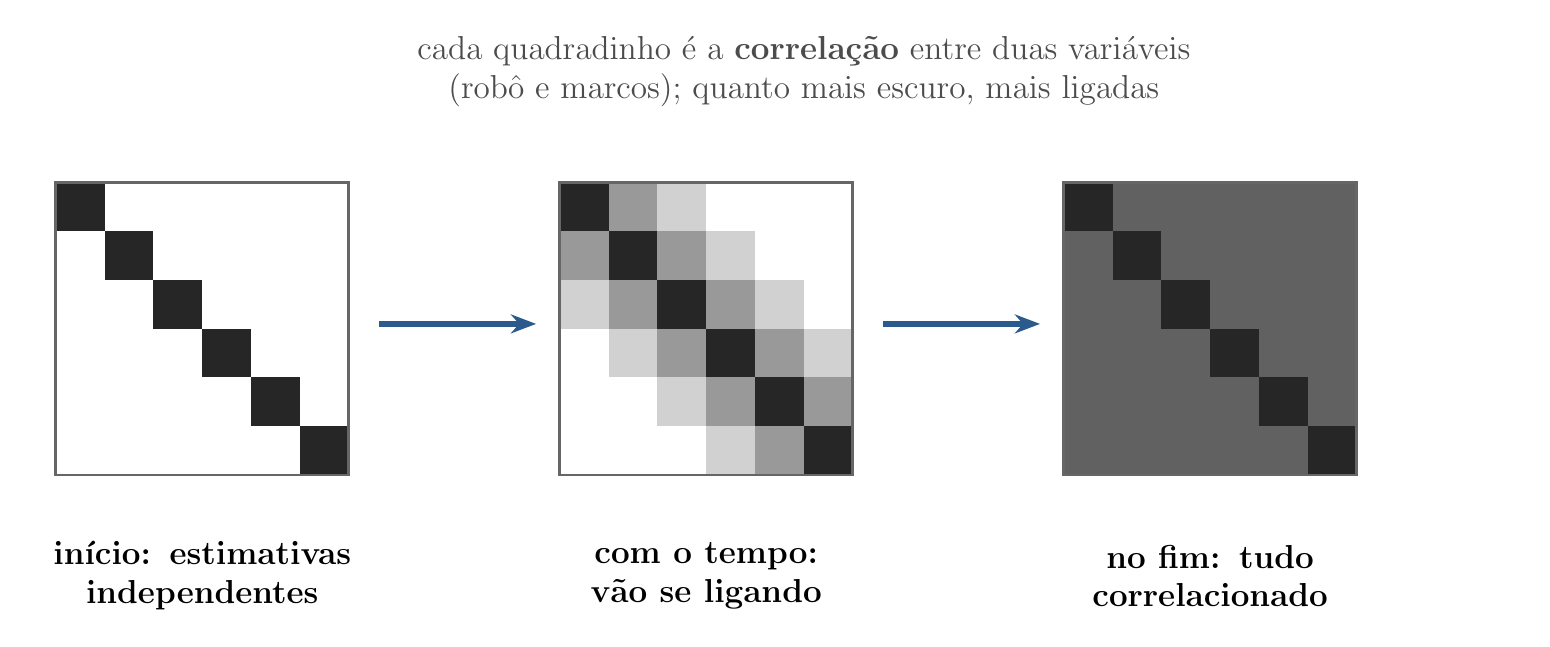
\begin{tikzpicture}[x=1cm,y=1cm]
\fill[black!85] (0.0,4.38) rectangle (0.62,5.0);
\fill[black!0] (0.62,4.38) rectangle (1.24,5.0);
\fill[black!0] (1.24,4.38) rectangle (1.86,5.0);
\fill[black!0] (1.86,4.38) rectangle (2.48,5.0);
\fill[black!0] (2.48,4.38) rectangle (3.1,5.0);
\fill[black!0] (3.1,4.38) rectangle (3.72,5.0);
\fill[black!0] (0.0,3.76) rectangle (0.62,4.38);
\fill[black!85] (0.62,3.76) rectangle (1.24,4.38);
\fill[black!0] (1.24,3.76) rectangle (1.86,4.38);
\fill[black!0] (1.86,3.76) rectangle (2.48,4.38);
\fill[black!0] (2.48,3.76) rectangle (3.1,4.38);
\fill[black!0] (3.1,3.76) rectangle (3.72,4.38);
\fill[black!0] (0.0,3.14) rectangle (0.62,3.76);
\fill[black!0] (0.62,3.14) rectangle (1.24,3.76);
\fill[black!85] (1.24,3.14) rectangle (1.86,3.76);
\fill[black!0] (1.86,3.14) rectangle (2.48,3.76);
\fill[black!0] (2.48,3.14) rectangle (3.1,3.76);
\fill[black!0] (3.1,3.14) rectangle (3.72,3.76);
\fill[black!0] (0.0,2.52) rectangle (0.62,3.14);
\fill[black!0] (0.62,2.52) rectangle (1.24,3.14);
\fill[black!0] (1.24,2.52) rectangle (1.86,3.14);
\fill[black!85] (1.86,2.52) rectangle (2.48,3.14);
\fill[black!0] (2.48,2.52) rectangle (3.1,3.14);
\fill[black!0] (3.1,2.52) rectangle (3.72,3.14);
\fill[black!0] (0.0,1.9) rectangle (0.62,2.52);
\fill[black!0] (0.62,1.9) rectangle (1.24,2.52);
\fill[black!0] (1.24,1.9) rectangle (1.86,2.52);
\fill[black!0] (1.86,1.9) rectangle (2.48,2.52);
\fill[black!85] (2.48,1.9) rectangle (3.1,2.52);
\fill[black!0] (3.1,1.9) rectangle (3.72,2.52);
\fill[black!0] (0.0,1.28) rectangle (0.62,1.9);
\fill[black!0] (0.62,1.28) rectangle (1.24,1.9);
\fill[black!0] (1.24,1.28) rectangle (1.86,1.9);
\fill[black!0] (1.86,1.28) rectangle (2.48,1.9);
\fill[black!0] (2.48,1.28) rectangle (3.1,1.9);
\fill[black!85] (3.1,1.28) rectangle (3.72,1.9);
\draw[black!60, line width=1pt] (0.0,1.28) rectangle (3.72,5.0);
\fill[black!85] (6.4,4.38) rectangle (7.02,5.0);
\fill[black!40] (7.02,4.38) rectangle (7.64,5.0);
\fill[black!18] (7.64,4.38) rectangle (8.26,5.0);
\fill[black!0] (8.26,4.38) rectangle (8.88,5.0);
\fill[black!0] (8.88,4.38) rectangle (9.5,5.0);
\fill[black!0] (9.5,4.38) rectangle (10.12,5.0);
\fill[black!40] (6.4,3.76) rectangle (7.02,4.38);
\fill[black!85] (7.02,3.76) rectangle (7.64,4.38);
\fill[black!40] (7.64,3.76) rectangle (8.26,4.38);
\fill[black!18] (8.26,3.76) rectangle (8.88,4.38);
\fill[black!0] (8.88,3.76) rectangle (9.5,4.38);
\fill[black!0] (9.5,3.76) rectangle (10.12,4.38);
\fill[black!18] (6.4,3.14) rectangle (7.02,3.76);
\fill[black!40] (7.02,3.14) rectangle (7.64,3.76);
\fill[black!85] (7.64,3.14) rectangle (8.26,3.76);
\fill[black!40] (8.26,3.14) rectangle (8.88,3.76);
\fill[black!18] (8.88,3.14) rectangle (9.5,3.76);
\fill[black!0] (9.5,3.14) rectangle (10.12,3.76);
\fill[black!0] (6.4,2.52) rectangle (7.02,3.14);
\fill[black!18] (7.02,2.52) rectangle (7.64,3.14);
\fill[black!40] (7.64,2.52) rectangle (8.26,3.14);
\fill[black!85] (8.26,2.52) rectangle (8.88,3.14);
\fill[black!40] (8.88,2.52) rectangle (9.5,3.14);
\fill[black!18] (9.5,2.52) rectangle (10.12,3.14);
\fill[black!0] (6.4,1.9) rectangle (7.02,2.52);
\fill[black!0] (7.02,1.9) rectangle (7.64,2.52);
\fill[black!18] (7.64,1.9) rectangle (8.26,2.52);
\fill[black!40] (8.26,1.9) rectangle (8.88,2.52);
\fill[black!85] (8.88,1.9) rectangle (9.5,2.52);
\fill[black!40] (9.5,1.9) rectangle (10.12,2.52);
\fill[black!0] (6.4,1.28) rectangle (7.02,1.9);
\fill[black!0] (7.02,1.28) rectangle (7.64,1.9);
\fill[black!0] (7.64,1.28) rectangle (8.26,1.9);
\fill[black!18] (8.26,1.28) rectangle (8.88,1.9);
\fill[black!40] (8.88,1.28) rectangle (9.5,1.9);
\fill[black!85] (9.5,1.28) rectangle (10.12,1.9);
\draw[black!60, line width=1pt] (6.4,1.28) rectangle (10.12,5.0);
\fill[black!85] (12.8,4.38) rectangle (13.42,5.0);
\fill[black!62] (13.42,4.38) rectangle (14.04,5.0);
\fill[black!62] (14.04,4.38) rectangle (14.66,5.0);
\fill[black!62] (14.66,4.38) rectangle (15.28,5.0);
\fill[black!62] (15.28,4.38) rectangle (15.9,5.0);
\fill[black!62] (15.9,4.38) rectangle (16.52,5.0);
\fill[black!62] (12.8,3.76) rectangle (13.42,4.38);
\fill[black!85] (13.42,3.76) rectangle (14.04,4.38);
\fill[black!62] (14.04,3.76) rectangle (14.66,4.38);
\fill[black!62] (14.66,3.76) rectangle (15.28,4.38);
\fill[black!62] (15.28,3.76) rectangle (15.9,4.38);
\fill[black!62] (15.9,3.76) rectangle (16.52,4.38);
\fill[black!62] (12.8,3.14) rectangle (13.42,3.76);
\fill[black!62] (13.42,3.14) rectangle (14.04,3.76);
\fill[black!85] (14.04,3.14) rectangle (14.66,3.76);
\fill[black!62] (14.66,3.14) rectangle (15.28,3.76);
\fill[black!62] (15.28,3.14) rectangle (15.9,3.76);
\fill[black!62] (15.9,3.14) rectangle (16.52,3.76);
\fill[black!62] (12.8,2.52) rectangle (13.42,3.14);
\fill[black!62] (13.42,2.52) rectangle (14.04,3.14);
\fill[black!62] (14.04,2.52) rectangle (14.66,3.14);
\fill[black!85] (14.66,2.52) rectangle (15.28,3.14);
\fill[black!62] (15.28,2.52) rectangle (15.9,3.14);
\fill[black!62] (15.9,2.52) rectangle (16.52,3.14);
\fill[black!62] (12.8,1.9) rectangle (13.42,2.52);
\fill[black!62] (13.42,1.9) rectangle (14.04,2.52);
\fill[black!62] (14.04,1.9) rectangle (14.66,2.52);
\fill[black!62] (14.66,1.9) rectangle (15.28,2.52);
\fill[black!85] (15.28,1.9) rectangle (15.9,2.52);
\fill[black!62] (15.9,1.9) rectangle (16.52,2.52);
\fill[black!62] (12.8,1.28) rectangle (13.42,1.9);
\fill[black!62] (13.42,1.28) rectangle (14.04,1.9);
\fill[black!62] (14.04,1.28) rectangle (14.66,1.9);
\fill[black!62] (14.66,1.28) rectangle (15.28,1.9);
\fill[black!62] (15.28,1.28) rectangle (15.9,1.9);
\fill[black!85] (15.9,1.28) rectangle (16.52,1.9);
\draw[black!60, line width=1pt] (12.8,1.28) rectangle (16.52,5.0);
\draw[dtrans, line width=2pt, -{Stealth[length=3.2mm]}] (4.1,3.2) -- (6.1,3.2);
\draw[dtrans, line width=2pt, -{Stealth[length=3.2mm]}] (10.5,3.2) -- (12.5,3.2);
\node[font=\large\bfseries, text width=4.2cm, align=center] at (1.86,0.0) {início: estimativas \textbf{independentes}};
\node[font=\large\bfseries, text width=4.2cm, align=center] at (8.26,0.0) {com o tempo: \textbf{vão se ligando}};
\node[font=\large\bfseries, text width=4.2cm, align=center] at (14.66,0.0) {no fim: \textbf{tudo correlacionado}};
\node[font=\large, black!70, text width=18cm, align=center] at (9.5,6.4) {cada quadradinho é a \textbf{correlação} entre duas variáveis (robô e marcos); quanto mais escuro, mais ligadas};
\end{tikzpicture}
\end{document}
